\section{Programming Language Performance}


There is often a debate in industry about the efficiency of programming languages, as the execution efficiency of a program often represents the performance of the program. For the same hardware conditions, a programming language that executes more efficiently often means greater load, lower latency, which is reflected in the real world as a better user experience and lower cost. The debate about programming language performance has been going on since the dawn of computing, but when it comes to performance today, most people tend to agree that C++ has higher performance than Java, and that C++ should be used to write high-performance computing because of its high performance. This is not wrong, but most people don't understand what they are talking about when they talk about the performance of programming languages. There are many factors that affect the performance of a programming language, and one cannot simply assume that one language has higher performance than another, especially if there is a specific application scenario, and the performance of a programming language is often closely related to the setting of the scenario. This leads to the concept of benchmarking.

Benchmarking provides a way to systematically test the performance differences of different individuals under the same category, providing a basis for scientifically judging individual merits. Generally in computer science, benchmarking refers to the evaluation of the performance of an object by running a particular computer program or a particular behavior of some operation, usually through a series of comparative experiments with controlled variables usually involving several iterative rounds in order to draw reproducible and precise conclusions. In addition, it focuses on a particular program and should exclude the influence of unrelated programs on the benchmark test, which requires that the benchmark test should have a clear idea of the underlying workings and avoid errors due to state uncertainty of the system. Benchmarking was first applied to computer hardware in computing, a common example being the floating-point performance of GPUs. But in recent years it can also be used for computer software, for example benchmarking compilers and databases.

\subsection{Factors affecting the performance of programming languages}

In terms of impact coverage alone, compilation principles have the greatest impact on the efficiency of programming languages. In industrial applications, the performance bottleneck in most scenarios is compile-related, where compile refers to compile in a broad sense, including not only compile-time but also run-time. The impact of compilation on programming language efficiency is again multifaceted. First, for the same programming language, using different compilers often results in different target codes and thus different runtime efficiencies, often because of different compile-time optimizations. For example, for C++, the Clang-LLVM compilation method has a significant performance difference at runtime compared to the target code obtained by using the GCC compilation method. Second, for the same programming language, it can be compiled not only in AOT (Ahead Of Time) way, but also in JIT (Just In Time) way. For example, for Kotlin, it can be compiled not only as bytecode to run on JVM, but also as JavaScript code to run on the browser, or even in Kotlin Native, compiled into native code. In this way, the different compilation methods have a greater impact on efficiency.


\begin{figure}[htbp]
    \centerline{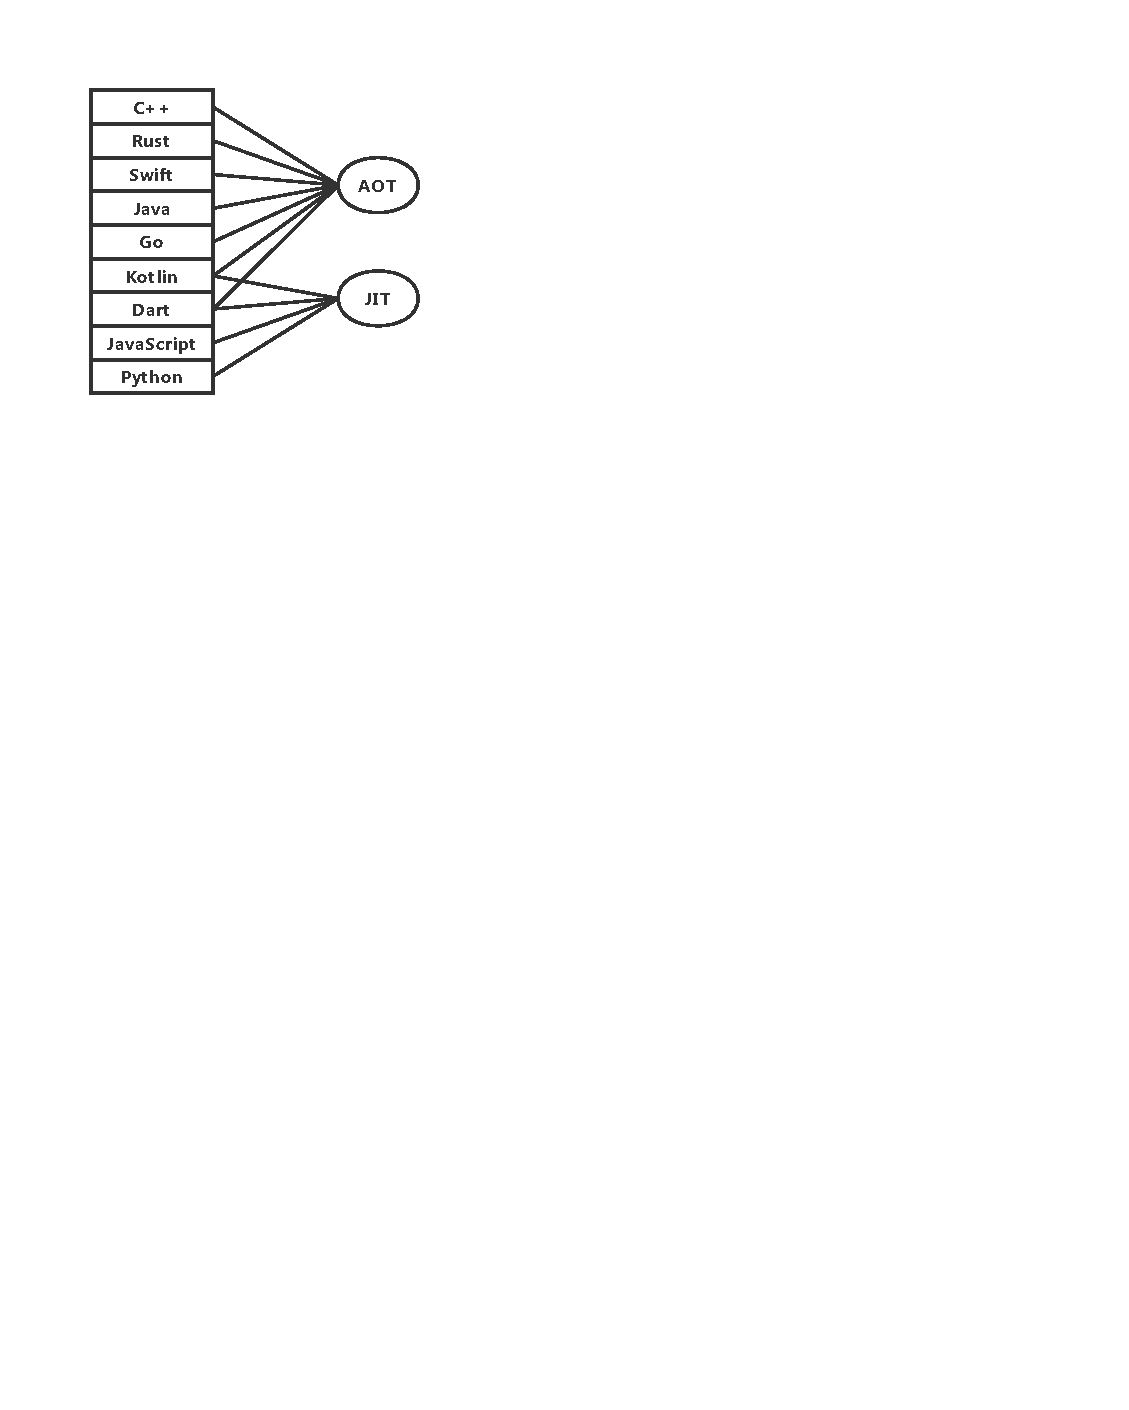
\includegraphics[scale=0.8]{figures/compilation}}
    \caption{compilation}
    \label{fig:compilation}
\end{figure}

Memory management, although not obvious in everyday use, actually has a huge impact on programming language performance. First, there is the matter of memory allocation on the heap. For languages with virtual machines, memory memory is a big advantage compared to non-VM languages. This is because VM languages tend to provide memory pools that host memory allocation, whereas non-VM languages do not have such an advantage. Of course, for scenarios where on-heap memory is used frequently, non-VM languages tend to use custom or third-party provided memory pooling frameworks, and the performance gap in industry is not as pronounced. Similarly, for VM languages, managed memory pools are not all good, and when memory jitter occurs, VMs perform frequent GCs, which also affects performance. Second, there is the principle of locality about memory. If the memory is accessed sequentially, the CPU will put all the adjacent data into the Cache, which greatly improves the hit rate of the Cache and thus the performance. Also with the compiler's loop unfolding optimization, higher efficiency is achieved. If the memory is accessed randomly, the performance is greatly reduced.

\begin{figure}[htbp]
    \centerline{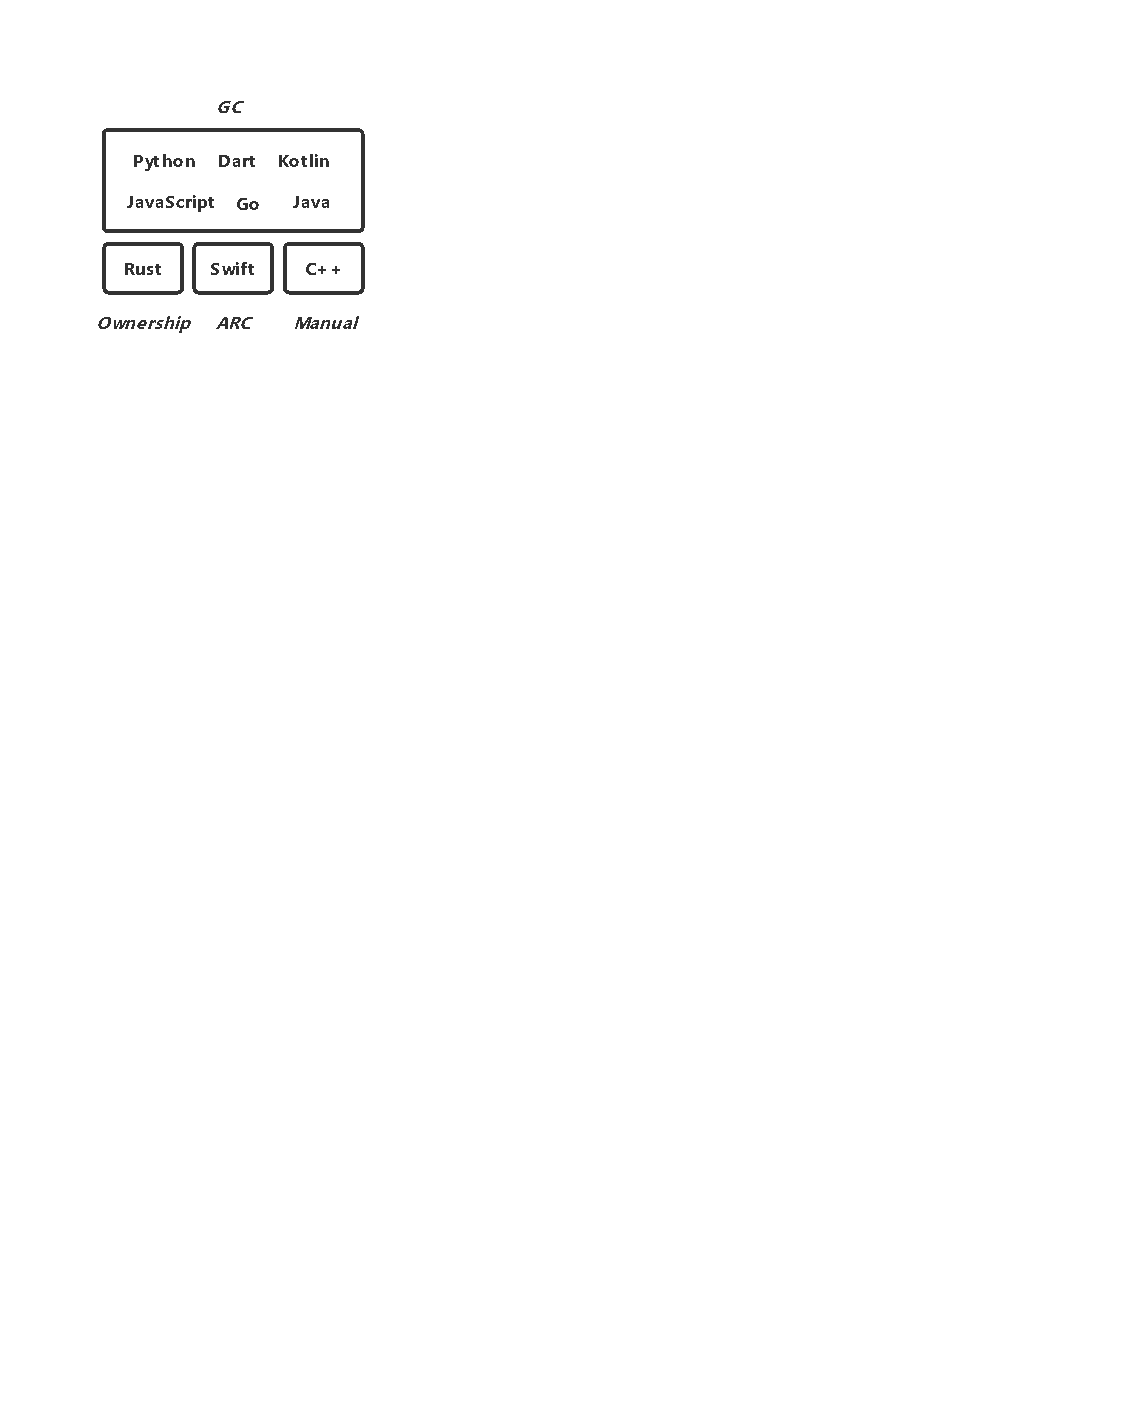
\includegraphics[scale=0.8]{figures/memory}}
    \caption{memory}
    \label{fig:memory}
\end{figure}

\subsection{Benchmarking Setup}

The dynamic metrics of the Computer Language Benchmarking Game are derived from the ideas of one of the more popular cross-language benchmarking suites available today, the Computer Language Benchmarking Game. The Computer Language Benchmarking Game currently consists of 10 benchmarking programs. Each of them provides a completely different problem for which different language specifications, language features and methods are used in an attempt to solve them using the most general way.

In this test, coarse-grained batch testing is performed uniformly using Python scripts, using built-in process tools to invoke Linux system commands, without relying on third-party libraries. It has high testing efficiency and is suitable for testing large amounts of data. Execution is performed six times for each test program and averaged to avoid errors. Each benchmark test was executed with larger and smaller scale inputs. The parameters of the testbed used, see table. The compilation parameters of the programming language, see Table.

Come for the same language with different compilers or compilation methods, the differences brought by the different compilation methods are compared (e.g. C++, Dart). The remaining languages are classified according to the programming language type system and execution method. Because for multiple languages with the same type system and compilation method, there should be an overlap in their scope of application in practice, the comparative analysis.


\begin{table}[ht]
    \caption{version}
    \label{tab:version}
    \begin{center}
        \begin{tabular}{ccc}
            \toprule
            Language   & Version         & Dependency \\
            \midrule
            Python     & CPython3.8      &            \\
            Java       & OpenJDK17       &            \\
            C++        & Clang14/GCC11.2 &            \\
            JavaScript & Node16          &            \\
            Go         & Go1.17          &            \\
            Swift      & Swift5.5        &            \\
            Dart       & Dart2.16        &            \\
            Rust       & Rust1.54        & MinGW7.3   \\
            Kotlin     & Kotlin1.6       & OpenJDK8   \\
            \bottomrule
        \end{tabular}
    \end{center}
\end{table}


For each language, there are 4 test metrics, which are:

\begin{enumerate}
    \item Compiler. Marked after the programming language, if not marked then the official compiler is used.
    \item gzip. gzip is a transfer compression protocol commonly used in industry. It is used to represent the size of the source code after compression. For the same algorithm, the smaller the amount of code used in a given programming language, the more syntactically expressive the language can be considered, in general.
    \item Time. The amount of time required to run the algorithm. Expressed as the minimum value of multiple runs. Includes startup time.
    \item Memory. The peak space consumption to run the algorithm. Expressed as the maximum of multiple runs.
\end{enumerate}

\subsection{binary-trees}

The idea is derived from Hans-J. Boehm's GC bench algorithm. The memory allocation capacity and garbage collection capacity are measured by repeatedly allocating and reclaiming space in large quantities. The steps are as follows.

\begin{figure}[htbp]
    \centerline{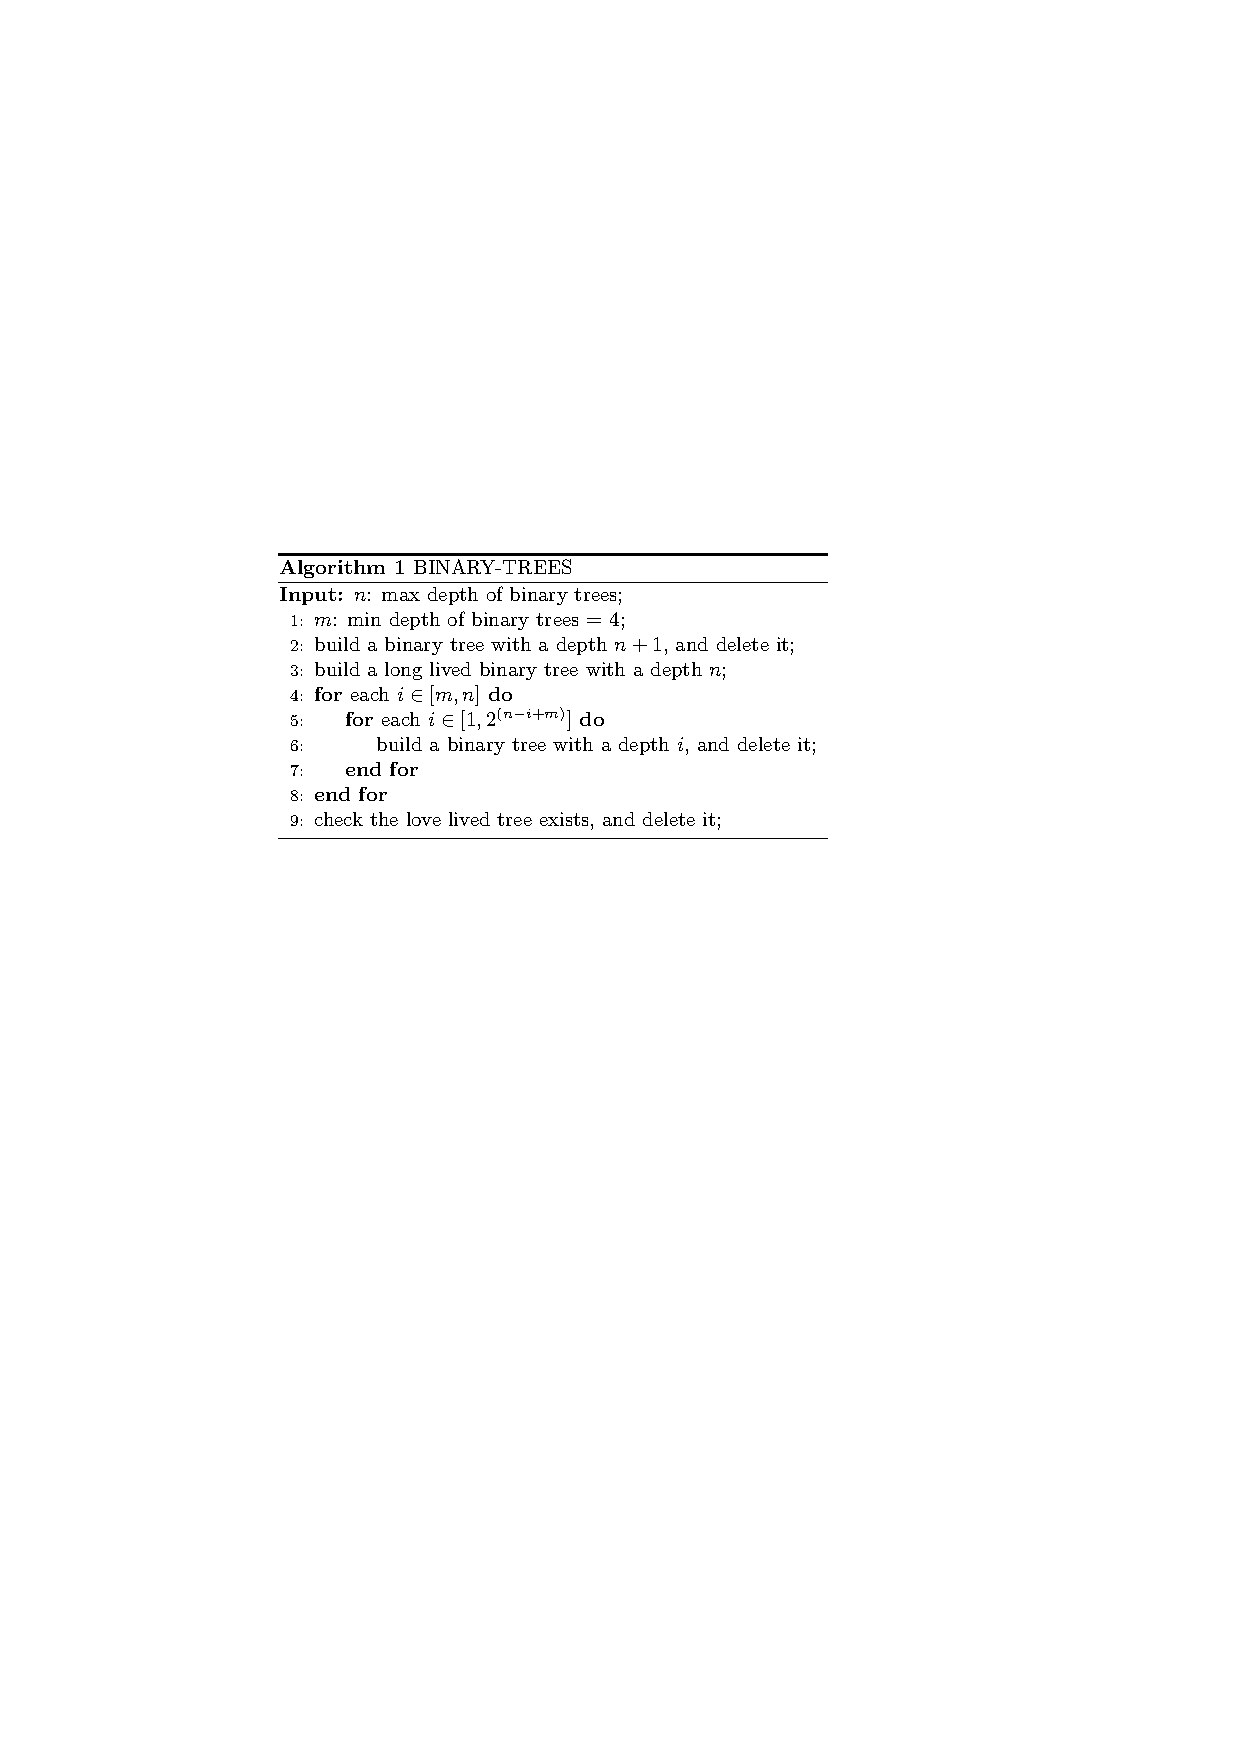
\includegraphics[scale=0.8]{figures/binary-trees}}
    \caption{binary-trees}
    \label{fig:binary-trees}
\end{figure}


\begin{table}[ht]
    \caption{binary-trees-1}
    \label{tab:binary-trees-1}
    \begin{center}
        \begin{tabular}{lrrrr}
            \toprule
            {}        & n  & size(B) & cpu(s)  & mem(KB) \\
            lang      &    &         &         &         \\
            \midrule
            cpp-clang & 21 & 654     & 16.438  & 263580  \\
            cpp-gcc   & 21 & 654     & 22.181  & 263620  \\
            dart-aot  & 21 & 1212    & 45.461  & 799012  \\
            dart-jit  & 21 & 1212    & 61.531  & 1626352 \\
            go        & 21 & 482     & 50.955  & 220548  \\
            java      & 21 & 552     & 5.607   & 2015512 \\
            js-node   & 21 & 711     & 36.391  & 1130788 \\
            kt-jvm    & 21 & 494     & 8.923   & 1783144 \\
            python3   & 21 & 589     & 169.912 & 442180  \\
            rust      & 21 & 751     & 7.796   & 132508  \\
            swift     & 21 & 714     & 63.608  & 733144  \\
            \bottomrule
        \end{tabular}
    \end{center}
\end{table}

\begin{table}[ht]
    \caption{binary-trees-2}
    \label{tab:binary-trees-2}
    \begin{center}
        \begin{tabular}{lrrrr}
            \toprule
            {}        & n  & size(B) & cpu(s) & mem(KB) \\
            lang      &    &         &        &         \\
            \midrule
            cpp-clang & 14 & 654     & 0.087  & 1200    \\
            cpp-gcc   & 14 & 654     & 0.104  & 3928    \\
            dart-aot  & 14 & 1212    & 0.120  & 1680    \\
            dart-jit  & 14 & 1212    & 0.644  & 170008  \\
            go        & 14 & 482     & 0.214  & 7232    \\
            java      & 14 & 552     & 0.155  & 47968   \\
            js-node   & 14 & 711     & 0.717  & 90512   \\
            kt-jvm    & 14 & 494     & 0.249  & 36040   \\
            python3   & 14 & 589     & 0.911  & 14420   \\
            rust      & 14 & 751     & 0.042  & 1176    \\
            swift     & 14 & 714     & 0.299  & 17616   \\
            \bottomrule
        \end{tabular}
    \end{center}
\end{table}

As you can see from the table, Java has the best memory allocation and management speed among these programming languages, and it takes very little time. However, Java's memory consumption is relatively the largest among these languages. This is due to the unique memory model of the JVM, which divides the heap area into different generations and uses different garbage collection algorithms for each generation. The advantage of this is obvious, it can greatly reduce the efficiency of garbage collection. But at the same time, it takes up more memory than is actually needed for the division. Since Kotlin and Java are both based on the JVM, they have similar performance figures. Kotlin is based on Java8, while Java is based on Java17. From Java9 onwards, the default JVM GC is G1. Parallel has a better response time than Parallel, but also consumes more memory. This is in perfect agreement with the data in the table that Kotlin has a slightly higher time overhead than Java and a slightly lower memory overhead than Java.

For the two different compilers for C++, Clang and GCC, the memory overheads are almost identical. This is because both of them manage memory manually. Clang, however, has a lower time consumption than GCC. This comes from the compiler optimizations, which are better in Clang than in GCC. The compiler architecture of Clang-LLVM is different. Clang-LLVM uses a low-coupling front- and back-end architecture, while GCC uses a front- and back-end coupling architecture, due to the fact that GCC is relatively old and limited by its age. This shows that compile-time optimization of the compiler is more important for a native compiled language.

Rust, Go, and Swift, which are also modern strongly typed, compiled languages, use three different memory management models. Go uses a garbage collection mechanism. Although Go is a compiled language, it has an additional runtime to support garbage collection. Compared to Java, Go uses a more conservative garbage collection strategy and does not adopt a drastic space-for-time strategy, resulting in a decent space consumption and a less optimistic runtime for memory allocation. Rust, on the other hand, uses an ownership mechanism that differs from the purely manually managed C/C++ and from Go's garbage collection. In terms of the underlying implementation, Rust does not actually maintain a runtime to manage space, but rather determines the timing of reclaiming memory at compile time through a complex arithmetic ownership algorithm. As a result, Rust's memory management is overhead-free. In fact, Rust's compiler backend uses LLVM, the same backend as the Clang-LLVM group tested above, and it is also clear from the test data that Rust performs almost identically to Cpp-Clang on floating-point operations. However, due to its ownership mechanism, Rust is better in memory allocation. For Swift, the memory management mechanism is different from all of the above. swift allocates and reclaims memory by maintaining a runtime reference count. In addition, Swift forces reference counts to be updated atomically instead of Rust's compiler management of thread safety, which results in high CPU overhead. This shows that Swift has a higher runtime overhead compared to Rust, confirming the data that Swift performs poorly compared to Rust.

\subsection{n-body}

The idea comes from the Symplectic Integration algorithm of K. P. Rauch and D. P. Hamilton simulates the evolution of multiple planets and confirms the correctness of the algorithm by checking the energy of each evolutionary state.

The performance bottleneck is mainly focused on floating-point operations. The steps are as follows.

\begin{figure}[htbp]
    \centerline{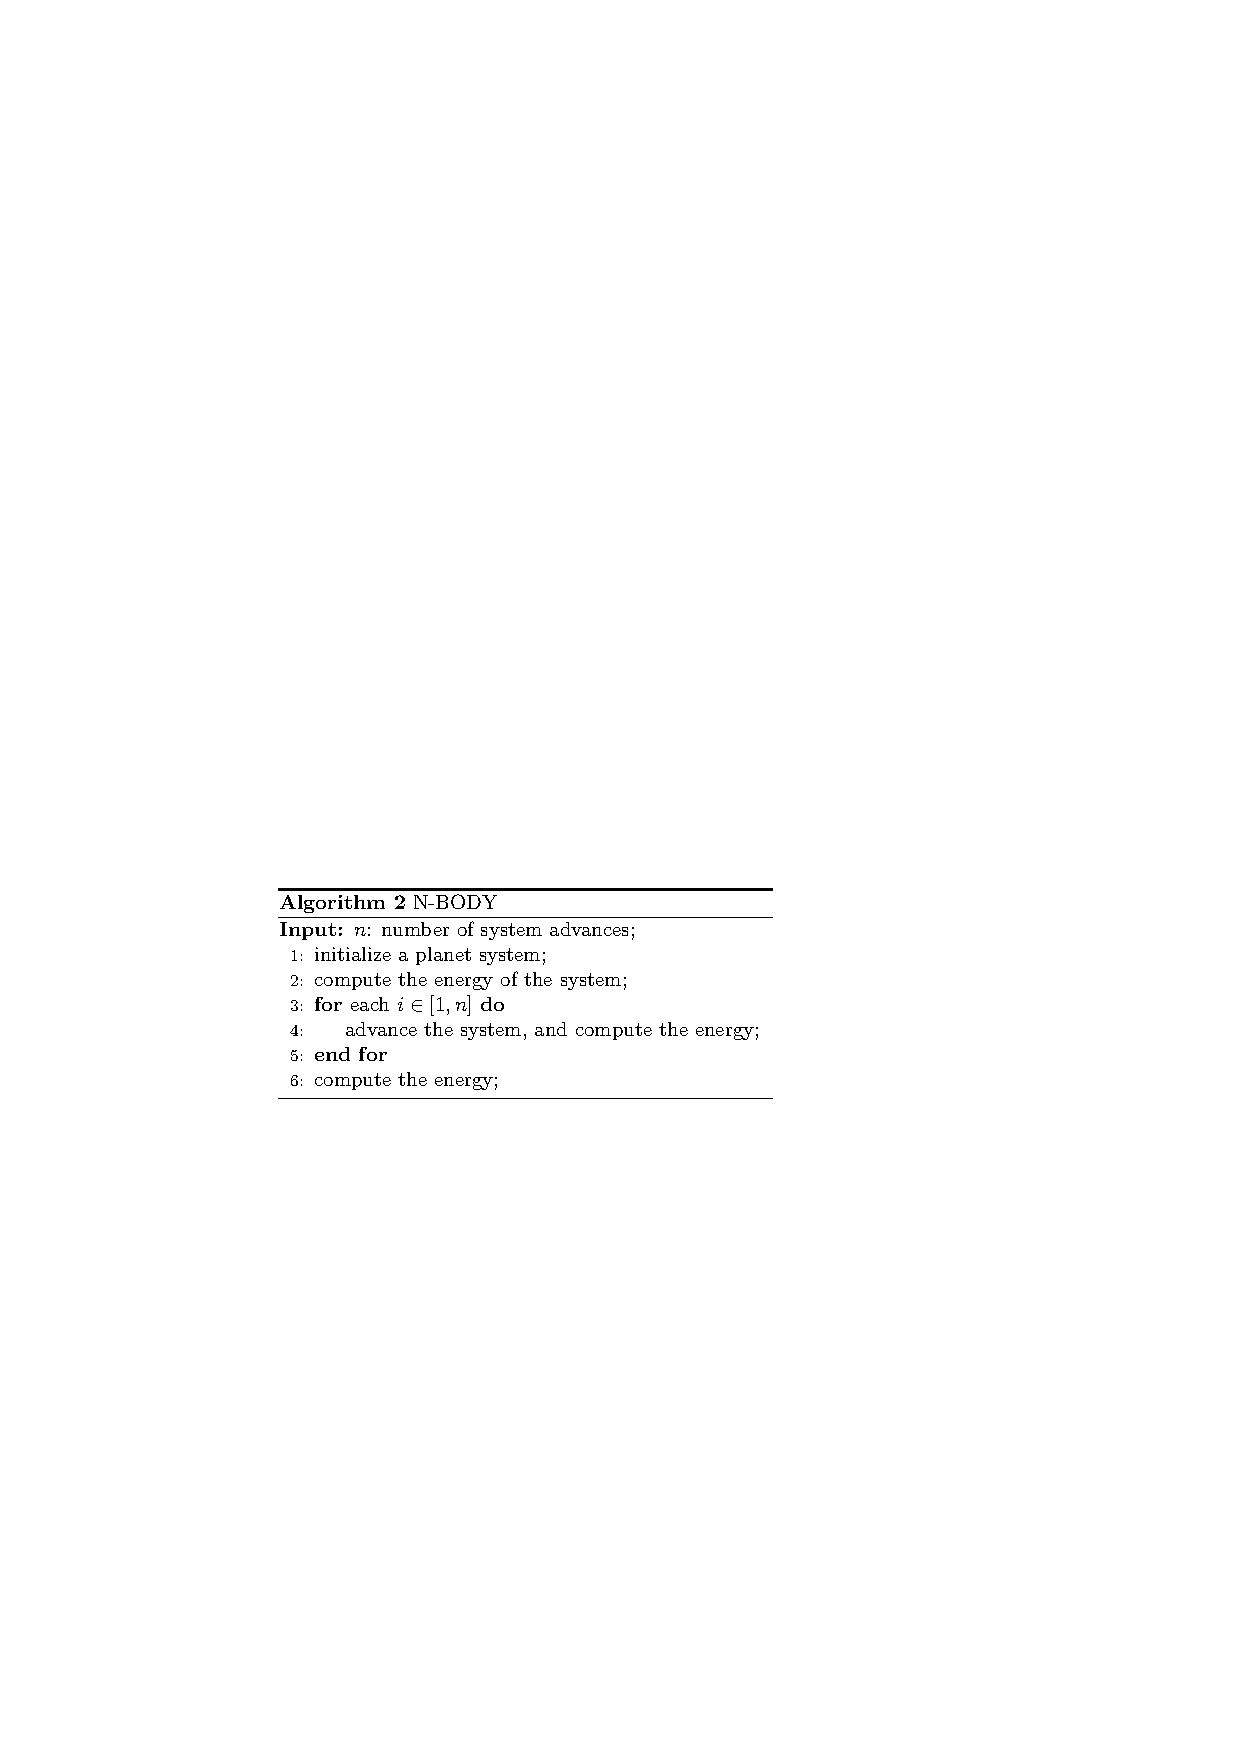
\includegraphics[scale=0.8]{figures/n-body}}
    \caption{n-body}
    \label{fig:n-body}
\end{figure}

\begin{table}[ht]
    \caption{n-body-1}
    \label{tab:n-body-1}
    \begin{center}
        \begin{tabular}{lrrrr}
            \toprule
            {}        & n        & size(B) & cpu(s)  & mem(KB) \\
            lang      &          &         &         &         \\
            \midrule
            cpp-clang & 50000000 & 1173    & 5.926   & 1236    \\
            cpp-gcc   & 50000000 & 1173    & 7.555   & 1228    \\
            dart-aot  & 50000000 & 1266    & 10.220  & 9308    \\
            dart-jit  & 50000000 & 1266    & 13.193  & 143436  \\
            go        & 50000000 & 1310    & 6.581   & 1128    \\
            java      & 50000000 & 1430    & 7.816   & 37260   \\
            js-node   & 50000000 & 1268    & 8.550   & 39956   \\
            kt-jvm    & 50000000 & 1124    & 6.914   & 37068   \\
            python3   & 50000000 & 1196    & 541.319 & 7780    \\
            rust      & 50000000 & 1480    & 5.818   & 1024    \\
            swift     & 50000000 & 1192    & 9.585   & 6308    \\
            \bottomrule
        \end{tabular}
    \end{center}
\end{table}


\begin{table}[ht]
    \caption{n-body-2}
    \label{tab:n-body-2}
    \begin{center}
        \begin{tabular}{lrrrr}
            \toprule
            {}        & n       & size(B) & cpu(s) & mem(KB) \\
            lang      &         &         &        &         \\
            \midrule
            cpp-clang & 5000000 & 1173    & 0.621  & 1204    \\
            cpp-gcc   & 5000000 & 1173    & 0.766  & 1204    \\
            dart-aot  & 5000000 & 1266    & 1.033  & 9216    \\
            dart-jit  & 5000000 & 1266    & 1.918  & 143256  \\
            go        & 5000000 & 1310    & 0.661  & 816     \\
            java      & 5000000 & 1430    & 0.880  & 37460   \\
            js-node   & 5000000 & 1268    & 0.941  & 39864   \\
            kt-jvm    & 5000000 & 1124    & 0.826  & 37064   \\
            python3   & 5000000 & 1196    & 52.530 & 7800    \\
            rust      & 5000000 & 1480    & 0.579  & 1020    \\
            swift     & 5000000 & 1192    & 0.976  & 6308    \\
            \bottomrule
        \end{tabular}
    \end{center}
\end{table}


Java's time consumption is not very high and does not fall too far behind native compiled languages. The performance bottleneck of algorithmic programs with short total runtime in Java is mainly the JVM startup time and the JIT-optimized warm-up time, and for algorithms that are already warmed up, Java's execution speed does not lag behind that of native compiled languages. Java runs in two steps. In the first step, the source code is compiled into bytecode, and in the second step, the JVM interprets and executes the bytecode. In the process of interpreting and executing the bytecode, JVM will receive the runtime information of the set code, and if it finds that some bytecode is executed more frequently, it will choose to compile this part of bytecode into native code, and call the native code directly when it is executed again. The so-called performance optimization of Java is mainly focused on the compilation stage of bytecode, while the source-to-bytecode stage is only simply optimized.

There is a significant performance gap between JavaScript and Python, and JavaScript has excellent performance with Google's V8 engine, which executes js code much like the Java virtual machine executes bytecode, using the same JIT optimization technology, so compared to Python, which does not use JIT optimization, it So compared to Python, which does not use JIT optimization, it has a huge performance improvement, and even has a similar floating-point performance to Java and native compiled languages. In fact, the speed of scripting languages is not a performance bottleneck in most application scenarios. However, in recent years, JavaScript has become the "assembly of the web", and more and more languages are being compiled into JavaScript, such as Kotlin, Dart, etc. As a result, more and more business logic needs to be executed in JavaScript, which makes This makes JavaScript burdened with tedious business-related logic, and the trend is to optimize JavaScript.

\subsection{mandelbrot}

\begin{figure}[htbp]
    \centerline{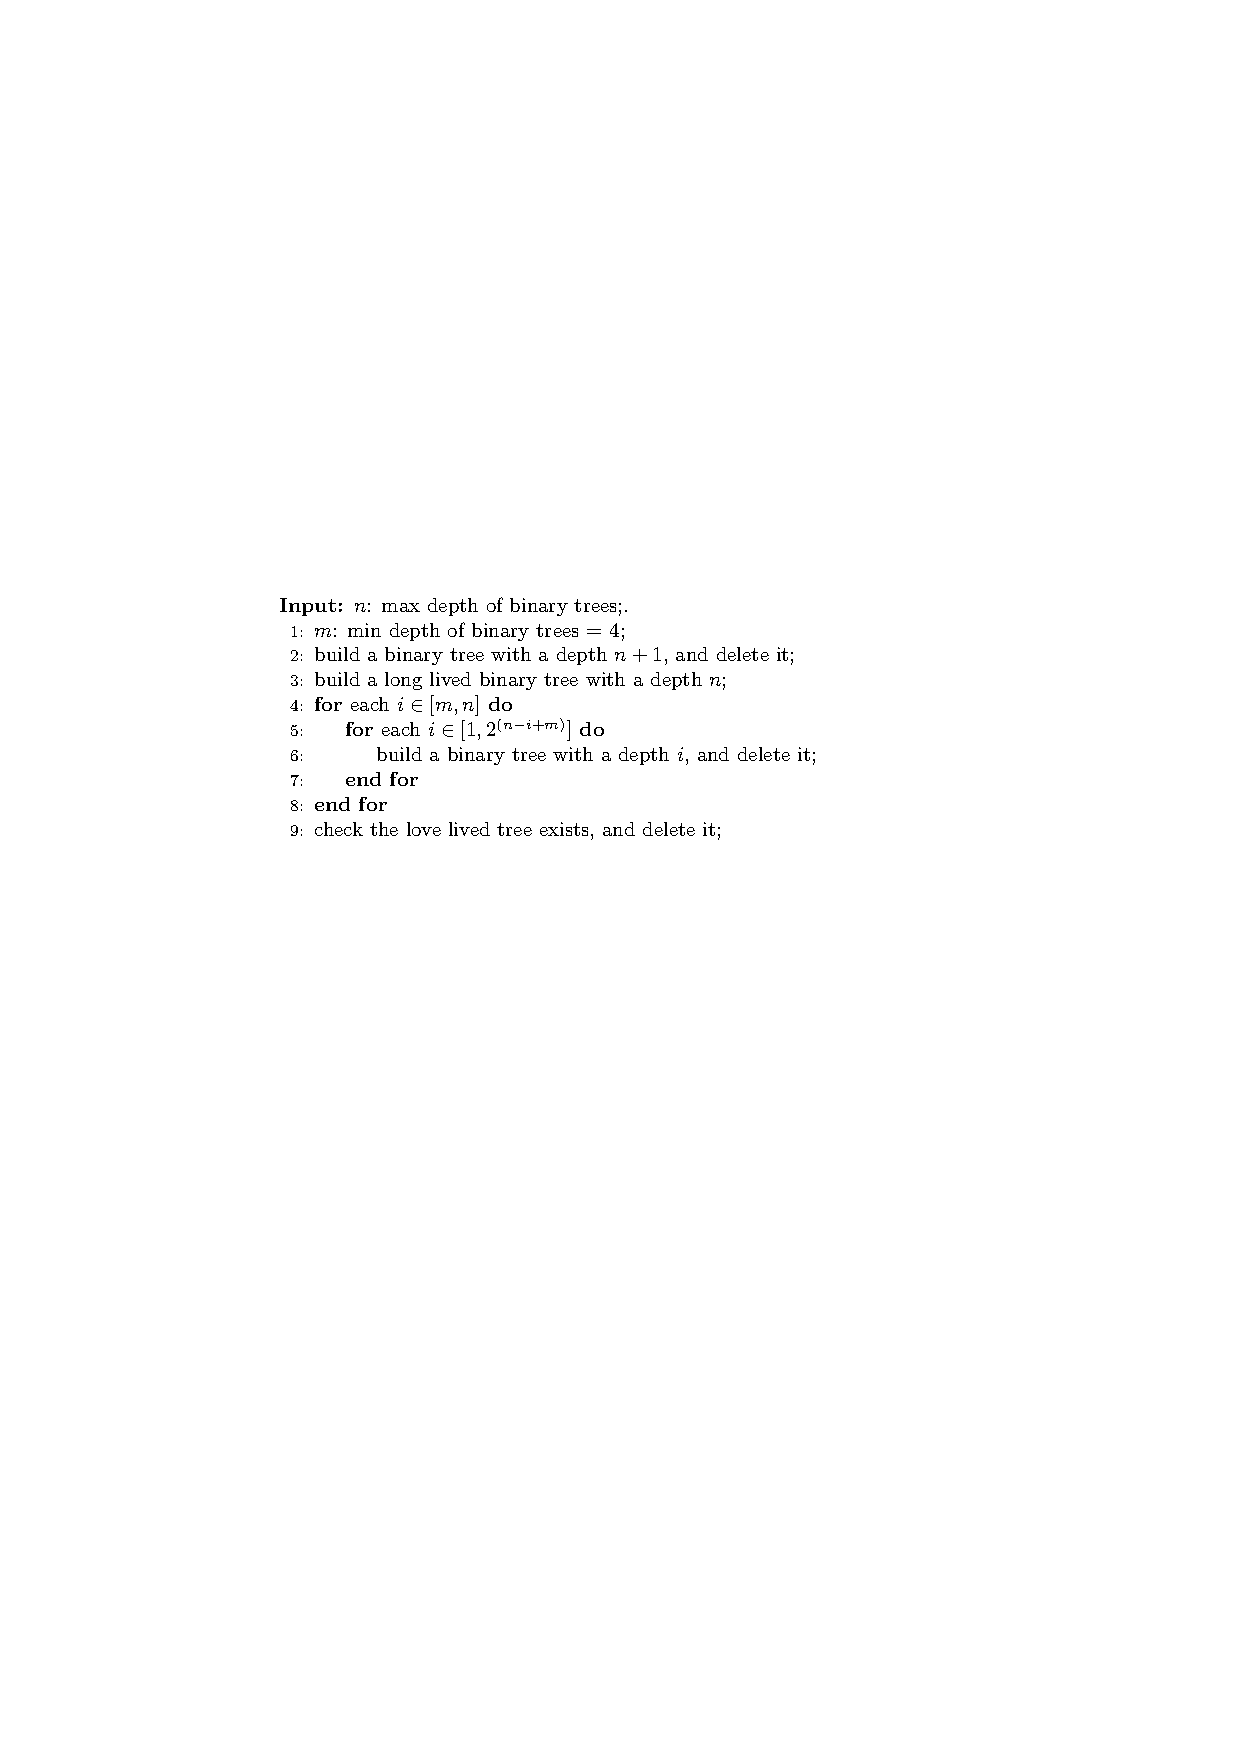
\includegraphics[scale=0.8]{figures/mandelbrot}}
    \caption{mandelbrot}
    \label{fig:mandelbrot}
\end{figure}

\begin{table}[ht]
    \caption{mandelbrot-1}
    \label{tab:mandelbrot-1}
    \begin{center}
        \begin{tabular}{lrrrr}
            \toprule
            {}        & n     & size(B) & cpu(s)  & mem(KB) \\
            lang      &       &         &         &         \\
            \midrule
            cpp-clang & 16000 & 822     & 13.900  & 30172   \\
            cpp-gcc   & 16000 & 822     & 13.931  & 28696   \\
            dart-aot  & 16000 & 454     & 154.089 & 17240   \\
            dart-jit  & 16000 & 454     & 151.501 & 148144  \\
            go        & 16000 & 823     & 19.598  & 32412   \\
            java      & 16000 & 665     & 27.834  & 34264   \\
            js-node   & 16000 & 373     & 130.638 & 42020   \\
            kt-jvm    & 16000 & 407     & 30.032  & 28432   \\
            python3   & 16000 & 688     & 702.599 & 47780   \\
            rust      & 16000 & 868     & 11.904  & 38528   \\
            swift     & 16000 & 394     & 26.277  & 6200    \\
            \bottomrule
        \end{tabular}
    \end{center}
\end{table}


\begin{table}[ht]
    \caption{mandelbrot-2}
    \label{tab:mandelbrot-2}
    \begin{center}
        \begin{tabular}{lrrrr}
            \toprule
            {}        & n    & size(B) & cpu(s) & mem(KB) \\
            lang      &      &         &        &         \\
            \midrule
            cpp-clang & 4000 & 822     & 0.880  & 1552    \\
            cpp-gcc   & 4000 & 822     & 0.881  & 1192    \\
            dart-aot  & 4000 & 454     & 10.276 & 17380   \\
            dart-jit  & 4000 & 454     & 10.096 & 148084  \\
            go        & 4000 & 823     & 1.260  & 2420    \\
            java      & 4000 & 665     & 1.827  & 34352   \\
            js-node   & 4000 & 373     & 8.763  & 42540   \\
            kt-jvm    & 4000 & 407     & 2.419  & 28448   \\
            python3   & 4000 & 688     & 46.273 & 12172   \\
            rust      & 4000 & 868     & 0.757  & 4388    \\
            swift     & 4000 & 394     & 1.661  & 6240    \\
            \bottomrule
        \end{tabular}
    \end{center}
\end{table}

For the same Dart code, two different ways of compiling are used, JIT and AOT. For memory overhead, AOT has a definite advantage over JIT for both. While for time overhead, both have similar performance. This is caused by the compilation mechanism of Dart. In fact, the compilation and running mechanism of Dart is different from both the traditional way. The traditional AOT is to compile the program code directly into the target code on the target machine, which can be called and run independently by the operating system directly. However, for Dart, whether it is AOT or JIT, only the compilation time is different, and it will eventually be run on the virtual machine. In fact, when the compilation time is negligible, the time overhead of AOT and JIT is approximately equal. But this way of running has its unique disadvantage, it will significantly increase the running overhead of AOT mode, but this makes AOT compilation has a strong runtime support. Because of this feature, the Dart VM can save the current runtime state, and the next time the VM is started, it can directly load the last state without restarting. This is done mainly for a smooth development experience, and the incremental compilation feature allows the runtime results to change almost in real time as the code is changed, with minimal latency. This design is because Dart is mainly used as the development language for the front-end cross-platform framework Flutter, allowing real-time feedback on changes to the UI interface, which is difficult to do in other languages.


